\documentclass[tikz,border=5pt]{standalone}
\usepackage{amsmath}
\usetikzlibrary{arrows.meta, decorations.markings}
\usepackage{pgfplots}
\pgfplotsset{compat=1.11}
\usepgfplotslibrary{fillbetween}
\pgfdeclarelayer{bg}
\pgfsetlayers{bg,main}
\begin{document}
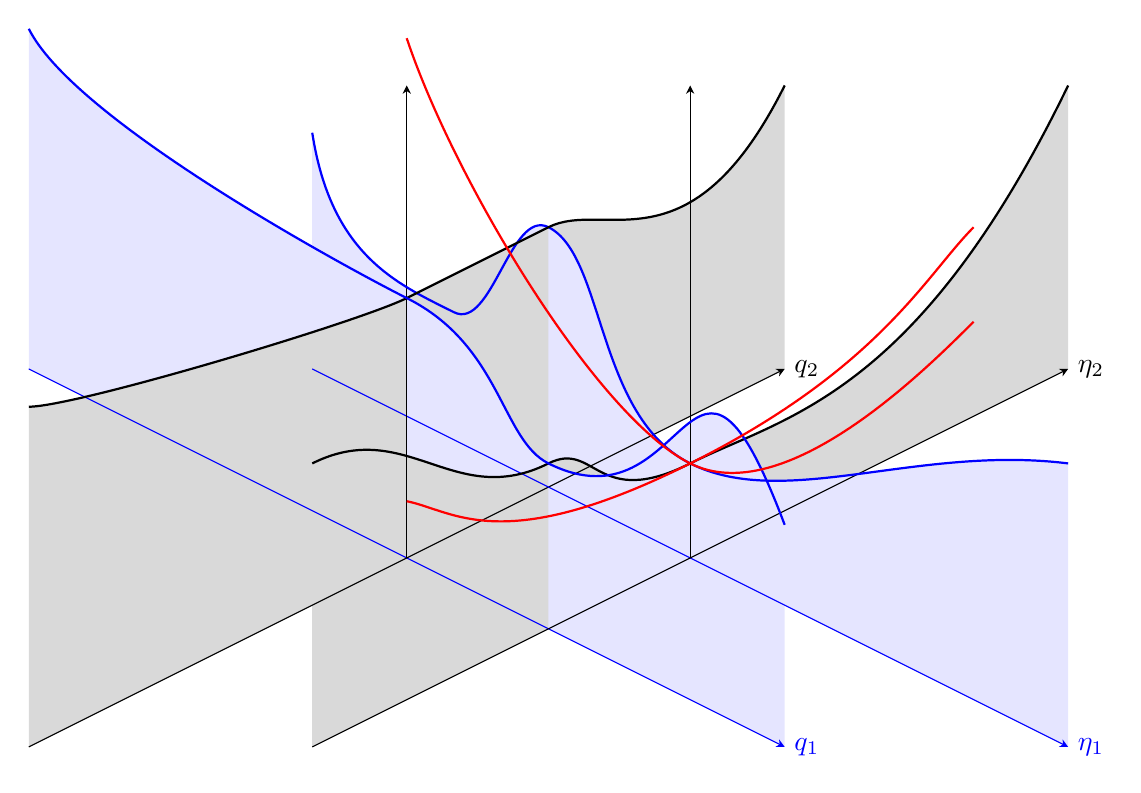
\begin{tikzpicture}[scale=1.2, >={Stealth[length=3pt,width=3pt]}]
\begin{pgfonlayer}{bg}
\fill[blue!10] (-1,4.5)--(-1,2)--(1.5,0.75)--(1.5,3.5) .. controls (1.1,3.7) and (0.9,2.4) .. (0.5,2.6)
.. controls (-0.1,2.9) and (-0.8,3.2) .. (-1,4.5);
\fill[blue!10] (-4,5.6)--(-4,2)--(0,0)--(0,2.75) .. controls (-0.5,3) and (-3.5,4.6) .. (-4,5.6);
\fill[black!15] (-4,1.6)--(-4,-2)--(4,2)--(4,5) .. controls (3,3) and (2.1,3.8) .. (1.5,3.5)
.. controls (1,3.25) and (0.5,3) .. (0,2.75) .. controls (-0.5,2.5) and (-3.5,1.6) .. (-4,1.6);
\fill[blue!10] (1.5,3.5)--(1.5,0.75)--(3,0)--(3,1) .. controls (2,1.5) and (2.1,3.2) .. (1.5,3.5);
\fill[blue!10] (0,2.75)--(0,0)--(1.5,-0.75)--(1.5,1) .. controls (1,1.25) and (1,2.25) .. (0,2.75);
\fill[black!15] (-1,1)--(-1,-2)--(7,2)--(7,5).. controls (5.4,1.7) and (4,1.5) .. (3,1)
.. controls (2,0.5) and (2,1.25) .. (1.5,1) .. controls (0.5,0.5) and (0,1.5) .. (-1,1);
\fill[blue!10] (3,1)--(3,0)--(7,-2)--(7,1).. controls (5.4,1.2) and (4,0.5) .. (3,1);
\fill[blue!10] (1.5,1)--(1.5,-0.75)--(4,-2)--(4,0.35).. controls (3,3) and (3,0.25) .. (1.5,1);
\draw[blue,->] (-4,2)--(4,-2)   node[right] {$q_1$};
\draw[->] (-4,-2)--(4,2) node[right] {$q_2$};
\draw[blue,->] (-1,2)--(7,-2) node[right] {$\eta_1$};
\draw[->] (-1,-2)--(7,2) node[right] {$\eta_2$};
\draw[->] (0,0)--(0,5);
\draw[->] (3,0)--(3,5);
\end{pgfonlayer}
\draw[blue,thick,-] (7,1)
.. controls (5.4,1.2) and (4,0.5) .. (3,1)%R
.. controls (2,1.5) and (2.1,3.2) .. (1.5,3.5)%MB
.. controls (1.1,3.7) and (0.9,2.4) .. (0.5,2.6)
.. controls (-0.1,2.9) and (-0.8,3.2) .. (-1,4.5);
\draw[thick,-] (7,5)
.. controls (5.4,1.7) and (4,1.5) .. (3,1)%R
.. controls (2,0.5) and (2,1.25) .. (1.5,1)%MO
.. controls (0.5,0.5) and (0,1.5) .. (-1,1);
\draw[thick,-] (4,5)
.. controls (3,3) and (2.1,3.8) .. (1.5,3.5)%MB
.. controls (1,3.25) and (0.5,3) .. (0,2.75)%L
.. controls (-0.5,2.5) and (-3.5,1.6) .. (-4,1.6);
\draw[blue,thick,-] (4,0.35)
.. controls (3,3) and (3,0.25) .. (1.5,1)%MO
.. controls (1,1.25) and (1,2.25) .. (0,2.75)%L
.. controls (-0.5,3) and (-3.5,4.6) .. (-4,5.6);
\draw[red,thick,-] (6,2.5)
.. controls (5.5,2) and (4,0.5) .. (3,1)
.. controls (2,1.5) and (0.5,4) .. (0,5.5);
\draw[red,thick,-] (6,3.5)
.. controls (5.5,3) and (5,2) .. (3,1)
.. controls (1,0) and (0.5,0.5) .. (0,0.6);
\end{tikzpicture}
\end{document}